Um den Algorithmus besser verstehen zu können, werden die Rahmenbedingungen formalisiert. Die Datenbank, besitzt $\mathbf{N}$ Elemente wobei  $\mathbf{N = 2^n}$ entspricht. Den Datensätzen ordnen wir die Elemente $\mathbf{ \{ 0,1 \}^n}$ zu. Wenn $\mathbf{ n=2}$ entspräche erhielt man die Elemente $\mathbf{00,01,10,11}$. Das gesuchte Elemente bezeichnen wir als  $\mathbf{\hat{x}}$. Die Datenbank wird als eine Funktion $\mathbf{f \{ 0,1 \}^n  \rightarrow \{ 0,1 \}}$ mit folgender Eigenschaft umgesetzt: \\
$\mathbf{f(x) = \begin{cases}1 \quad f\ddot{u}r \,
		x = \hat x \\0 \quad sonst \end{cases} 
}$ 
\newline
Mithilfe dieser Funktion haben wir unser Quantenorakel. $\mathbf{U_f : | x,y \rangle \to |x,y \oplus f(x) \rangle}$. Die Funktion $\mathbf{f}$gibt nur ein zurück, wenn die Eingabe das gesuchte Element $\mathbf{\hat x}$ ist. Das Quantenorakel, negiert daher nur das Vorzeichen des gesuchten Elements. 

\subsection{Prinzip}
Der Grover Algrothmus lässt sich in drei Schritte aufteilen.
\begin{enumerate}
	\item \textbf{Superpositionen aufbauen}
	\\
	im ersten Schritt werden alle Quantenbits in die Superposition gebracht.
	\item \textbf{Amplitudenveränderung durchführen} \emph{(Grover Iteration G)}
	\\
	Der Zweite Schritt verändert die Amplituden der Elemente. Dabei wird die Amplitude des gesuchten Elementes erhöht und alle anderen verringert. Dieser Schritt wird auch \emph{(Grover Iteration G)} genannt und abhängig von der Anzahl der Elementen öfters wiederholt. Wie oft die Grover Iteration ausgeführt werden muss, wird im Abschnitt \ref{sec:geoVer} erläutert.
	\item \textbf{Messen} 
	\\
	Im letzten Schritt werden die Quantenbits gemessen und man erhält mit einer hohen Wahrscheinlichkeit, das gesuchte Element $\mathbf{\hat x}$.
\end{enumerate}

\subsubsection{Amplitudenveränderung}
Die Amplitudenveränderung besteht aus zwei Schritten. Beim ersten Schritt handelt es sich um die Negation der Amplitude von $\mathbf{\hat x}$. Im zweiten Schritt wird die negative Amplitude ausgenutzt um die Amplitude zu verstärken. Dies passiert in dem alle Amplituden am Mittelwert aller Amplituden gespiegelt werden. 
\\ \\
\textbf{Negieren der Amplitude}
 \\
Um die Amplitude von $\mathbf{\hat x}$ zu negieren, wird ein Hilfsbit benötigt. Das Hilfsbit wird in den Zustand $\mathbf{H|1\rangle}$ mithilfe eines Hadamar Gatters gebracht. Dadurch erhalten wird $\mathbf{|x\rangle \frac{1}{\sqrt 2}(|0\rangle - |1\rangle )}$. Anschließend wird das Quantenorakel angewendet und damit das Vorzeichen der Amplitude des gesuchten Elementes negiert. Das Hilfsbit wird nun nicht mehr benötigt und kann in folgenden Berechnungen weggelassen werden. Dies lässt sich auch an folgender Abbildung erkennen. Dort ist Anwendung des Quantenorakel und beispielhaft die Amplituden alle Elemente der Datenbank vor und nach der Anwendung des Quantenorakels zu sehen.
\begin{figure}[hbtp]
	\centering
	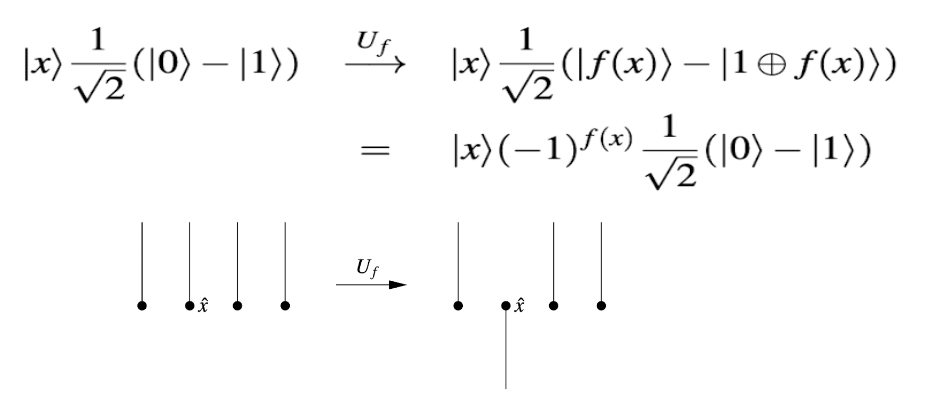
\includegraphics[width=.8\textwidth]{figures/amplitudenveraenderung.png}
	\caption{Amplitudenveränderung}
	\label{fig:changeAmplitude}
\end{figure}
Die negative Amplitude von $\mathbf{\hat x}$ hat keinen Einfluss auf das Messen, um mit einer erhöhten Wahrscheinlichkeit das Element $\mathbf{\hat x}$ nach dem Messen zu erhalten benötigt man den Schritt Spiegeln am Mittelwert.
\\\\
\textbf{Spiegelung am Mittelwert} \\
\label{sec:spiegelnAmMittelwert}
Um zu zeigen, das die Spiegelung der Amplituden am Mittelwert den gewünschten Effekt hat, folgen nun einige Beispiel Rechnungen. Eine Spiegelung an einem wert $\mathbf{m}$ entspricht der Abbildung: $\mathbf{\alpha \rightarrow 2 \times m - \alpha}$. \\
Nimmt man an die Datenbank enthält vier Elemente ($\mathbf{n=2}$) so entspricht - nach der Negation von $\mathbf{\hat x}$ - der Mittelwert $\mathbf{m = \frac{1}{4} \times (\frac{1}{2}- \frac{1}{2}+ \frac{1}{2} +\frac{1}{2}) = \frac{1}{4}}$. Die Spiegelung von $\mathbf{\hat x}$ entspricht $\mathbf{-\frac{1}{2} \times \frac{1}{4} - (-\frac{1}{2}) = 1}$. Damit ist die Amplitude des gesuchten Elements gleich eins. Würde man nun die Bits messen, erhält man mit einer Wahrscheinlichkeit von 100\% das Element $\mathbf{\hat x}$. Die Amplituden aller anderen Elemente entwickeln sich wie folgt: $\mathbf{\frac{1}{2} \times \frac{1}{4} - \frac{1}{2} = 0}$
\\ \\
Wäre $\mathbf{n = 3}$, so würde die Amplitude von $\mathbf{ \hat x}$ nach der ersten Grover Iteration $\mathbf{\frac{5}{5\sqrt 8}}$ und alle anderen Amplituden $\mathbf{\frac{1}{2\sqrt 8}}$ betragen. Nach einer Spiegelung am Mittelwert ist die Amplituden von $\mathbf{\hat x}$wieder positiv, bevor ein erneutes Spiegeln möglich ist um die Amplitiduen weiter zu verstärken oder zu verringern, muss zuerst erneut das Quantenorakel angewandt werden. Ein erneutes Spiegeln, nach der Negation, der Amplituden würde diese wie folgt verändern. Das gesuchte Element $\mathbf{\hat x}$ hätte eine Amplitude von $\mathbf{0,973}$, alle anderen Elemente eine von $\mathbf{-0, 088}$. Würde nun gemessen werden erhielte man mit einer Wahrscheinlichkeit von 93 \% das gesuchte Element.
\\ Ein erneutes Spiegeln würde die Amplituden des gesuchten Elementes  im Gegensatz zu Erwartung wieder verringern und alle anderen erhöhen, daher ist es besonders wichtig, dass nicht zu viele Grover Iterationen ausgeführt werden. Wie die Genaue Anzahl an Iterationen jedoch berechnet werden kann, folgt im Abschnitt \ref{sec:geoVer}
\textbf{SOUFFLE?}
\subsubsection{Graphische Darstellung des Grover Algorithmus}
Der Grover Algorithmus sieht nach dem bisherigen Erklärungen wie folgt aus.
\begin{figure}[hbtp]
	\centering
	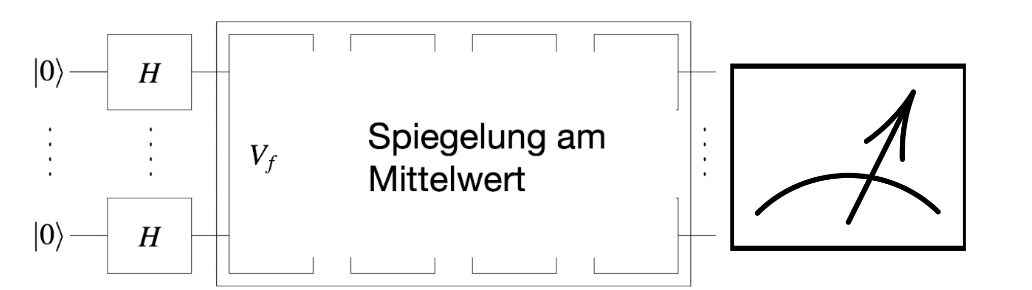
\includegraphics[width=1\textwidth]{figures/algotInformell.png}
	\caption{Graphische Darstellung des Grover Algorithmus \\ Quelle EIGENS ERSTELLEN!!!! }
	\label{fig:algotInformellt}
\end{figure}
Alle Bits werden mithilfe der Hadamar Gatter in Superpositionen gebacht. Alles danach bis zum Messen Symbol am Ende ist die Grover Iteration.
Der Äußere Kasten steht für das mehrfache Wiederholen dieser Iterationen. $\mathbf{V_f}$ steht für das Quantenorakel, jedoch wird hier das Hilfsbit nicht mit eingezeichnet.  Anschließend folgt die Spiegelung am Mittelt, wie diese genau mithilfe von Gattern umgesetzt wird folgt im nächsten Abschnitt \ref{sec:realiserung}. Nach dem ausführen der Grover Iterationen werden die Bits gemessen.
\subsection{Realisierung der Spiegelung am Mittelwert}
\label{sec:realiserung}
Die Abbildung $\mathbf{\alpha \rightarrow 2 \times m - \alpha}$ lässt sich mithilfe einer Matrixberechnung umsetzten.
\begin{center}
	$\mathbf{D_N \times 
	\begin{pmatrix}
			\alpha_0 & \alpha_1 & \dots &\alpha_{N-1}
	\end{pmatrix}^T, \text{mit } D_N = 
	\begin{pmatrix}
			-1 + \frac{2}{N} & \frac{2}{N} & \dots& \frac{2}{N} \\
			\frac{2}{N} & -1 \frac{2}{N} & \dots& \frac{2}{N} \\
			\vdots & \vdots & \ddots& \dots \\
			 \frac{2}{N} & \frac{2}{N} & \dots& -1+ \frac{2}{N} \\
	\end{pmatrix}}$
\end{center}
\subsubsection{Beispielrechnung}
Sei $\mathbf{N = 4}$ so ergibt sich folgende Rechnung:
\begin{center}
 $\mathbf{D_4  \times \begin{pmatrix}
		0,5 & -0,5 & 0,5 & 0,5
\end{pmatrix}^T}$.

$\mathbf{\begin{pmatrix}
		-0,5 & 0,5 &0,5&0,5\\
		0,5 & -0,5 &0,5&0,5\\
		0,5 & 0,5 &-0,5&0,5\\
		0,5 & 0,5 &0,5&-0,5
	\end{pmatrix}
	\times \begin{pmatrix} 0,5 \\ -0,5 \\ 0,5 \\ 0,5 \end{pmatrix} = \begin{pmatrix} 0\\1\\0\\0 \end{pmatrix}
}$.
\end{center}
Dieses Ergebnis gleicht sich mit dem Ergebnis aus Abschnitt \ref{sec:spiegelnAmMittelwert}, in dem wir ebenfalls alle Elemente einer Datenbank mit $\mathbf{N=4}$ Elementen an dem Mittelwert der Amplituden gespiegelt haben. Folgende Abbildung zeigt ebenfalls nochmal wie sich die Amplituden verändert haben.
\begin{figure}[hbtp]
	\centering
	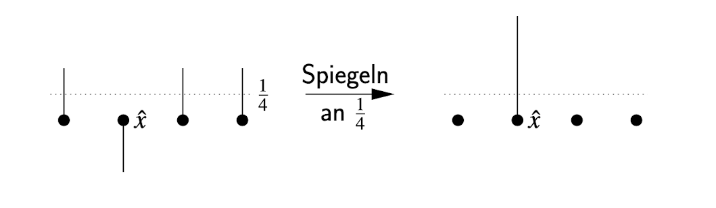
\includegraphics[width=.8\textwidth]{figures/spiegelung.png}
	\caption{Spiegelung am Mittelwert \\ Quelle: HOEMEISTER SEITE}
	\label{fig:spiegelung}
\end{figure}
Wenn eine $\mathbf{N \times N}$ Matrix verwendet wird, dann verstößt dies gegen das Lokalitätsprinzip. Daher muss die $\mathbf{D_n}$ Matrix in verschiedene unitäre Matrizen zerlegt werden.  $\mathbf{D_n}$ kann in ein Produkt aus drei unitäre Matrizen zerlegt werden.
\begin{center}
$\mathbf{D_n = -H_n \times R_N \times H_n, \text{mit } R  = 
\begin{pmatrix}
		-1 & 0 &\dots& 0 \\
		0& 1& \ddots& \vdots\\
		\vdots &\ddots& \ddots&0 \\
		0& \dots& 0 &1 \\
\end{pmatrix}}$
\end{center}
\subsubsection{Beispielrechnung}
Um zu zeigen, das die Matrix $\mathbf{D_N}$ wie oben als Produkt dreier Matrizen zerlegt werden kann, folgt ein Beispiel mit $\mathbf{D_4}$.
\begin{figure}[hbtp]
	\centering
	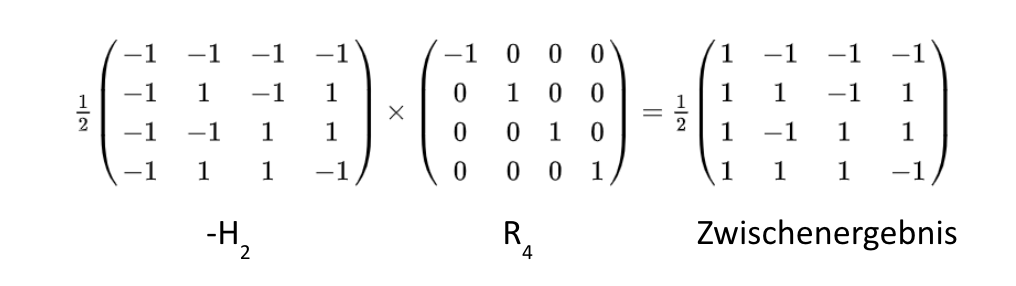
\includegraphics[width=.8\textwidth]{figures/householderLokal_1.png}
	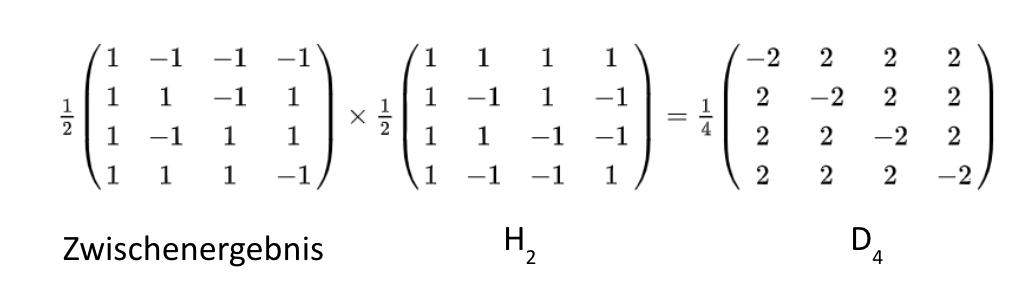
\includegraphics[width=.8\textwidth]{figures/householderLokal_2.png}
	\caption{Beispielzerlegung von $\mathbf{D_4}$ \\ Quelle: eigene Darstellung}
	\label{fig:DLokal}
\end{figure}
Das Ergebnis der Berechnung ist wie in der beschriftetet Rechnung \ref{fig:DLokal}) zu sehen gleich mit der zu erwarteten Matrix $\mathbf{D_4}$. Der Beweis, das dies auch für beliebige $\mathbf{N}$ zutrifft befindet sich in dem Buch vom Hoemeister auf der Seite 309 QUELLE.

\subsubsection{Matrix R als lokale Transformation}
Es wurde gezeigt, das die Matrix $\mathbf{D_N}$ in ein Produkt aus Matrizen zerlegt werden kann. Das die Hadamar Matrixen mit Hilfe eines Gattern als lokale Transformation umgesetzt werden können ist bekannt. Dies muss jedoch auch noch für $\mathbf{R_N}$ gezeigt werden. 
\\
Um ein Gatter zu entwickeln zu können, welches die Transformation $\mathbf{R_N}$ umsetzt, muss sich angeschaut werden wie sich $\mathbf{R_N}$ bei einer Multiplikation von Matrizen auswirkt. Alle Werte einer Matrix die mit $\mathbf{R_N}$ multipliziert wird bleiben gleich. Lediglich die erste Zeile oder Spalte wird negiert. Dies ist davon abhängig, ob die Matrix $\mathbf{R_N}$ auf der Linken oder Rechten Seite der Multiplikation ist. In ersten Zeile der Abbildung \ref{fig:DLokal} ist die Negation der ersten Spalte zu sehen.
\\
Multipliziert man $\mathbf{R_N}$ mit Amplituden, bedeutet dies, dass lediglich die Amplitude des ersten Elementes ($\mathbf{|0...0\rangle}$)negiert wird.
Falls $\mathbf{R_4}$ wäre, dann sähe das Gatter wie in Abbildung \ref{fig:Rgatter} aus.
 \begin{figure}[hbtp]
 	\centering
 	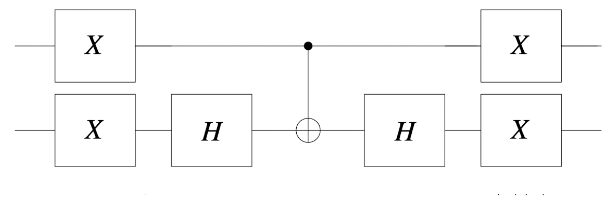
\includegraphics[width=.8\textwidth]{figures/rgatter.png}
 	\caption{$\mathbf{R_4}$ Realisierung \\ Quelle: HOEMEISTER SEITE}
 	\label{fig:Rgatter}
 \end{figure}
\\
Es folgt eine weitere Beispielrechnung, um zu verdeutlichen, das dieses Gatter die Transformation $\mathbf{R_4}$ ausführt.
\subsubsection{Beispielrechnung}
ABBILDUNG
 In den Abbildungen () werden die Werte der QBits $\mathbf{|00\rangle}$ und wie diese sich durch die einzelnen Gatter verändern dargestellt.
 Die Pauli X Gatter invertieren den Wert eines QBits. Aus $\mathbf{|0\rangle}$ wird $\mathbf{|1\rangle}$ und andersrum. Das erste Bit wird bis zum letzten Pauli-X Gatter nicht mehr verändert. Es wird ausschließlich genutzt um zu schauen, ob das CNOT aktiviert wird. Das zweite QBit wird durch das erste Hadamar Gatter, in folgende Superposition $\mathbf{\frac{1}{\sqrt 2}(|0\rangle - |1\rangle)}$. Da das erste QBit den Wert $\mathbf{|1\rangle}$ hat wird das zweite QBit durch das CNOT negiert - $\mathbf{-\frac{1}{\sqrt 2}(|0\rangle - |1\rangle)}$. Anschließend durch läuft das zweite Bit wieder ein Hadamar Gatter, das QBit hat anschließend folgenden Wert: $\mathbf{-|1\rangle}$.
 Zum Schluss werden beide Bits ($\mathbf{|1\rangle}$ und $\mathbf{-|1\rangle}$) durch die Pauli-X Gatter invertiert und wir erhalten das gewünschte Ergebnis von $\mathbf{-|00\rangle}$.
  \\
  \\
  ABBILDUNG

 Die Abbildung () zeigt die QBits $\mathbf{|01\rangle}$  und wie diese von den Gattern verändert werden. Die ersten Pauli-X Gatter invertieren abermals die QBits, diese haben nun den Wert $\mathbf{|10\rangle}$. Das erste QBit wird bis auf von dem letzten Pauli-X Gatter nicht verändert und nur zur Aktivierung der Operation CNOT zuhilfe genommen. Das zweite QBit wird durch das Hadamar Gatter in die Superpostion $\mathbf{\frac{1}{\sqrt 2}(|0\rangle + |1\rangle)}$ gebracht. Diese verändert sich auch nicht durch die CNOT Operation. Nach der CNOT Operation wird das QBit durch das zweite Hadamar Gatter wieder in den Basiszustand $\mathbf{|0\rangle}$ gebracht. Zuletzt durchlaufen die beiden QBits ein Pauli-X Gatter welches die QBits von den Basiszustände $\mathbf{|10\rangle}$ in den erwarteten Zustand $\mathbf{|01\rangle}$ überführt. Die QBits haben nach dem durchlaufen des Gatters die selben Zustände wie vorher.
  \\ 
  \\
Bei den QBits $\mathbf{|10\rangle \text{ und }|11\rangle}$, wird die CNOT Operation nicht ausgeführt, da das erste QBit in den Basiszustand $\mathbf{|0\rangle}$ überführt werden. Die QBits werden durch die doppelte Ausführung der Gatter ebenfalls nicht verändert.
\\
\\
Daran kann gesehen werden, dass die Gatter die gewünschte Operation $\mathbf{R_4}$ ausführen.

\subsection{Graphische Darstellung des Grover Algorithmus}
In der Abbildung() ist wie in der Abbildung() der Grover Algorithmus nochmals Graphisch dargestellt. Dieses mal enthält die Abbildung alle verschiedenen Gatter, die die QBits durchlaufen.



